\section*{Bitter Lesson}

\begin{frame}
  \frametitle{The Bitter Lesson}
  \vfill
  \centering
  \begin{minipage}{0.88\textwidth}
    \Large\itshape
    ``The biggest lesson that can be read from 70 years of AI research is that
    \textcolor<2->{searchcolor}{general methods that leverage computation}
    are ultimately the most effective, and by a large margin.''
  \end{minipage}
  \vfill
  \source{Rich Sutton, ``The Bitter Lesson'', March 13, 2019}
  \vfill
\end{frame}

\begin{frame}
  \frametitle{What Scales?}
  \vfill
  \centering
  \only<1>{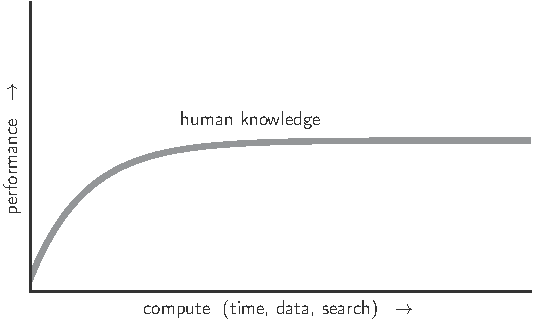
\includegraphics[width=0.9\textwidth]{s0-bitter-curve-human}}%
  \only<2>{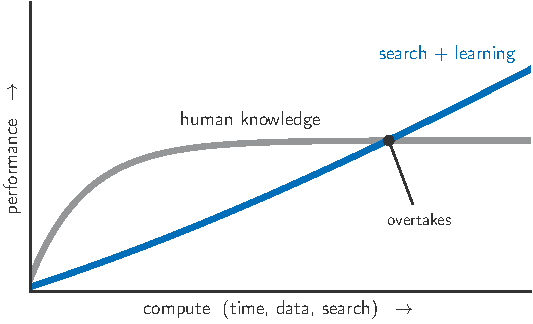
\includegraphics[width=0.9\textwidth]{s0-bitter-curve}}%
  \vfill
  \source{Schematic illustration, not measured data}
\end{frame}

\begin{frame}
  \frametitle{Search and Learning}
  \vfill
  \centering
  \begin{tikzpicture}[x=1cm, y=1cm]
    \node[rlbox=humancolor, minimum width=4.8cm, minimum height=2.4cm, font=\Large] (hk)
    {\textbf{Contains}\\what we discovered};
    \node[rlbox=searchcolor, minimum width=4.8cm, minimum height=2.4cm, font=\Large, right=0.6cm of hk] (sl)
    {\textbf{Discovers}\\from experience};
    \node[font=\Large\bfseries, above=5pt of hk] {Human knowledge};
    \node[font=\Large\bfseries, text=searchcolor!85!black, above=5pt of sl] {Search + Learning};
  \end{tikzpicture}
  \vfill
  \keyidea{Learning from self experience is the entire thesis of RL.}
\end{frame}
